% Template PNSAC newsletter - Article
% Language: Latex
%

% Head

\title{Project Manager's Progress Report}
\subtitle{October 2013}
\author{Bruce Gemmill}

\maketitle

\section{Nr 3 Engine}
\label{sec:engines_3}

Engine 3 is almost completely reassembled, with only the supercharger
and intercooler preheat assemblies left to install on the engine,
which was moved to the QEC engine frame in early summer.  The work has
slowed somewhat, due to summer down time for staff and volunteers, but
we continue to make steady progress.

The auxiliary gearbox was recently removed from the engine firewall,
and is now being disassembled.  This is the last major assembly that
must be overhauled before the engine can be installed on the aircraft.

\section{Engine Frame}
\label{engineframe}

Now that the engine and frame are joined, the major work still
required is rebuilding the many cowl panels and the radiator flaps
that surround the engine.  There is a lot of corrosion on the pieces,
and each must be disassembled, cleaned, then repaired before painting
and reassembly.  This work must be done carefully to ensure the cowl
panels fit properly when installed on the QEC.

This work has gone slowly due to the small number of volunteers who
are able to do this type of repair.


\section{Crew Lounge, Galley,  and Forward Washroom}
\label{crewlounge}

The new galley has now been installed in the crew lounge, and work
overhead in the ceiling is also complete.  This involved installing
new insulation and the Janitrol heaters, along with refurbished
heating ducts, and some new fuel lines.  The ceiling panels were also
installed.

The doors on the main electrical panel were restored and installed.
New circuit legend cards were produced to indicate the circuit breaker
and junction box connections.  These were laminated and installed
inside the electrical panels.  Some additional investigation is needed
to complete the electrical circuit connection diagrams that were badly
faded.

\begin{figure}[htbp]
   \vspace{2em}
   \centering
   %name of the graphic, without the path AND in EPS format:
   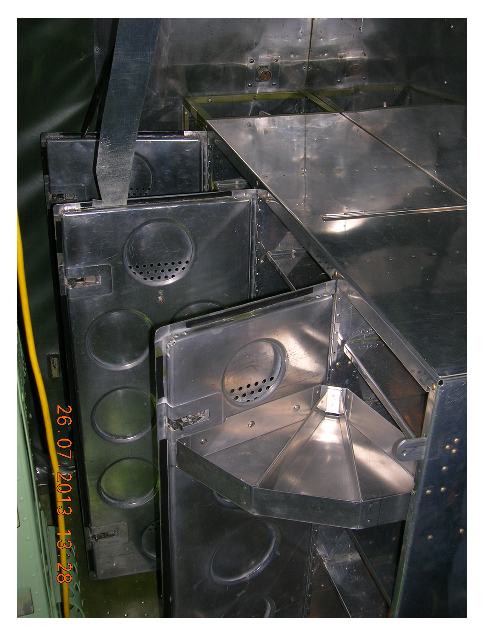
\includegraphics[scale=0.5]{galley_interior.eps}
   %caption of the figure 
   \caption*{\small \em New galley -- interior view.}
   %label of the figure, which has to correspond to \ref{}:
   \label{fig:galley_interior}
\end{figure}

One section of floor was patched after removing a corroded area.  One
additional repair needs to be done under the floor of the crew lounge.
Until this is complete, the new cushion flooring cannot be
installed. This has also delayed the installation of all of the crew
lounge accessories, such as the table, seats and secure storage bin,
all of which are complete but waiting in storage.


\section{Fuselage and Empennage}
\label{empenage}

The forward and rear belly compartments are now complete.  The two
battery elevators that were removed have been restored and installed
behind the nose wheel.  The battery compartment covers were repaired
but need painting and stencilling.

The firewall on nacelle 3 is being cleaned in preparation for the
installation of the engine sometime this winter.

Further progress has been made on the set of troop seats being
fabricated for the main cabin.


\section{Planned Restoration Work 2013/14}
\label{sec:plannedwork}

Over the next year, we hope to have engine Nr 3 completed and engine
Nr 4 removed.  We will complete the reassembly of the crew lounge and
galley.  We then plan to work on the main cargo compartment, including
refurbishing the main heater duct and other fittings, and removing
floors to begin cleaning and repairs under the cargo floor.  We may
yet get to work on the four engine nacelles.



\begin{footnotesize}
  \raggedleft PNSAC\\
\end{footnotesize}

% End of text.

%%% Local Variables: 
%%% mode: latex
%%% TeX-master: main_document.tex
%%% End: 

